%!TEX root = ./seminarpaper.tex

\chapter{Case Study: Linear Regression}

	% https://vincentarelbundock.github.io/Rdatasets/csv/Stat2Data/PorschePrice.csv

	This chapter shows an example in applied statistics, with the Student-T Distribution. Based on the value $t$ of the t-statistics and the value $\nu$, the number of degrees of freedom, the Student-T Distribution computes the probability, also known as p-value, that the null hypotheses is true. For the example, a data file \href{https://vincentarelbundock.github.io/Rdatasets/csv/Stat2Data/PorschePrice.csv}{\lstinline{PorschePrice.csv}} was used. That file contains the price of 30 different Porsches based on their age and mileage. The example is shown in listing \ref{lis:Porsche}. The first column contains the price of the car, the second one the age and the third and last column contains the mileage. The price is shown in 1000 U.S. dollar, the age in years and the mileage in 1000 miles.

	\begin{center}
		\begin{lstlisting}[caption={\lstinline{PorschePrice.csv} Example}, label={lis:Porsche}]
			"Price",	"Age",		"Mileage"
			69.4,		3,			21.5
			56.9,		3,			43
			49.9,		2,			19.9
			47.4,		4,			36
			42.9,		4,			44
			36.9,		6,			49.8
			83,			0,			1.3
			72.9,		0,			0.67
			69.9,		2,			13.4
			67.9,		0,			9.7
			66.5,		2,			15.3
			64.9,		2,			9.5
			58.9,		4,			19.1
			57.9,		3,			12.9
			54.9,		10,			33.9
			54.7,		11,			26
			53.7,		4,			20.4
			51.9,		4,			27.5
			51.9,		10,			51.7
			49.9,		3,			32.4
			44.9,		4,			44.1
			44.8,		13,			49.8
			39.9,		6,			35
			39.7,		6,			20.5
			34.9,		8,			62
			33.9,		7,			50.4
			23.9,		20,			89.6
			22.9,		22,			83.4
			16,			20,			86
			52.9,		3,			37.4
		\end{lstlisting}
	\end{center}

	To calculate the p-value of the given example, the \setlx\ program \href{https://raw.githubusercontent.com/karlstroetmann/Artificial-Intelligence/master/SetlX/simple-linear-regression.stlx}{\lstinline{simple-linear-regression.stlx}} from Karl Stroetmann is used. Some changes were made to fit the example. This program contains a procedure, that loads the \lstinline{PorschePrice.csv} file and returns it as an object of class \lstinline{Table} containing the values \lstinline{columnNames}, \lstinline{types} and \lstinline{data}. Another procedure will then extract the data from the object and store the values of the dependent variable in a list \lstinline{Y} and the value of the independent variable in a list \lstinline{X}. Based on these two lists, the two coefficients theta 0 ($\vartheta _0$) and theta 1 ($\vartheta _1$), the \ac{TSS}, the \ac{RSS}, the proportion of the explained variance $R^{2}$ and the value $t$ are computed. Based on $t$, the \ac{CDF} of the Student-T Distribution is calculated. Therefore, the implemented function \lstinline{stat_studentCDF()} is used. The explained variance and the p-value are printed in the console. To get an overview of the whole example, the program also plots the data. This is shown in figure \ref{fig:price_vs_age} and \ref{fig:price_vs_mileage}.

	\begin{figure}[h]
		\centering
		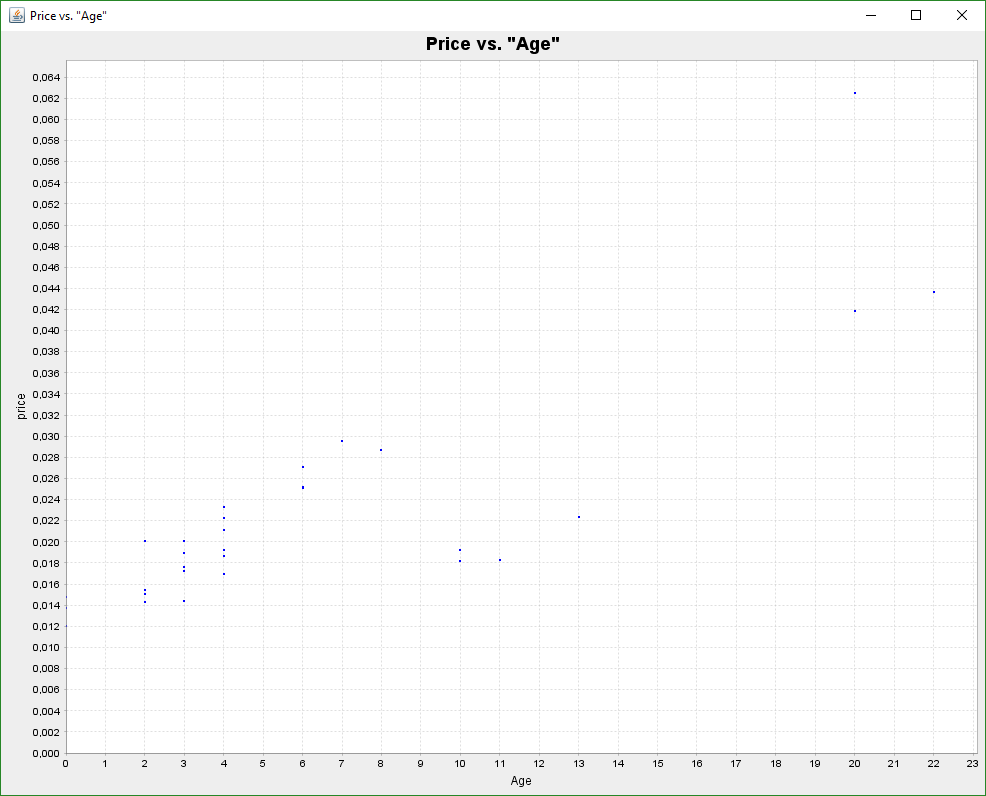
\includegraphics[width=1\textwidth]{Figures/price_vs_age}~\\
		\caption{Price vs. Age}
		\label{fig:price_vs_age}
	\end{figure}


	\begin{figure}[h]
		\centering
		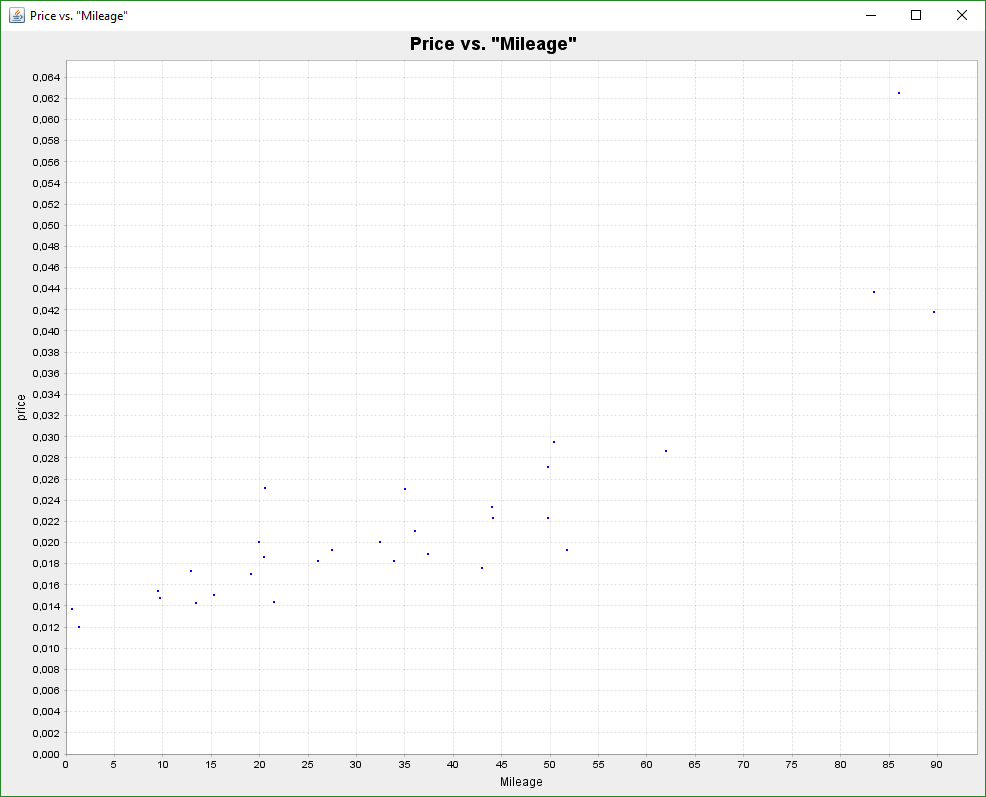
\includegraphics[width=1\textwidth]{Figures/price_vs_mileage}~\\
		\caption{Price vs. Mileage}
		\label{fig:price_vs_mileage}
	\end{figure}
